\subsection{Semantic Event Chains}
\label{ssec:action_methods_semanticeventchains}

One of the central goals of early human development is to recognize, learn, and lastly imitate actions.
Much in life is learned by imitation.
For example, a baby might look at her parents walking and try to imitate this behavior.
On the other side, a child might learn through unconscious imitation moral codes of society through the conduct of the parents, teachers, movies, or literature.
Another way of learning is by trial-and-error.
This method is used if no ready-made solution of a specific problem is available.
The learner performs random activities until the goal is reached accidentally.
A good example is given by younger children playing with wooden building blocks.
This type of undirected playing teaches to build small structures, \eg towers, and thus enable to learn physical properties.
Lastly, humans can learn by insight, which is the Gestalt view point.
According to this theory, solutions to a peculiar problem may appear sudden.
Because this type of learning does not consume much time, it is very important in the education field.
As example may serve a jar full of candy, sitting on a kitchen counter.
A child wants to reach the jar, but is too small.
The kid may sit down, think about the situation and come to the conclusion, that a chair can be used to reach the candy.

Similar to human beings, in cognitive robotics one of the central goals remains to recognize, learn, and lastly imitate actions.
However, it has been long addressed that naive observation and raw copying does not suffice to successfully perform an action by a robot~\cite{breazeal2002robots}.
If a human watches a pushing action, for example a pen pushed by a hand, he can bootstrap easily the essence of the action: The goal is to push the pen.
This action can be learned and repeated easily.
Here, it does not matter, if the left hand, right hand, or a tool is used, the essence is always still captured.
Even changes in trajectory or velocity can easily be applied.
It is suspected that the mirror-neuron system is involved in this feat; currently, it is not understood how newborns learn these advanced motor skills~\cite{rizzolatti2004mirror}.

For a robot however, it is even today difficult to tell, if a trajectory or a specific object is important to reach a certain goal.
This level of invariance is learned by human beings by relating actions with objects and which we call action understanding.
In~\cite{aksoy2011learning} a unified framework is introduced, which enables robots to classify, learn, and repeat actions.
\glsreset{ac:sec}This framework is called \glspl{ac:sec}.
A more detailed view is provided in~\cite{aksoy2012semantic}.
Semantic Event Chains store actions as a series of touching and non-touching events.

One example is given in \figref{fig:sec_secexample_blocksmarkednumbered}: Some wooden blocks are distributed on a table.
First, computer vision clusters, segments, and classifies the objects.
For visual purposes these steps were performed manually here.
We assume knowledge about ``up'' and ``down'' and say that the table is always below the objects.
This allows to extract a graph representation as shown in \figref{fig:sec_secexample_graph}.
In this graph there is the representation for \emph{touching} --- as seen in the example in the relation between block 1 and 3 --- and \emph{not touching} --- as seen in block 1 and 4.
The graph is undirected, unidirectional, and each edge is of unit length. 
Thus, the same graph can be represented in a symmetrical adjacency matrix as follows


\begin{figure}
  \centering
  \begin{subfigure}[t]{0.475\textwidth}
    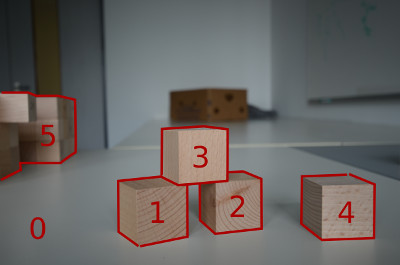
\includegraphics[width=\textwidth]{./figures/sec/secexample_blocksmarkednumbered.jpg}
    \subcaption{Manually segmented example scene of blocks on a table.}
    \label{fig:sec_secexample_blocksmarkednumbered}
  \end{subfigure}
  \hfill
  \begin{subfigure}[t]{0.475\textwidth}
    \raisebox{0.5cm}{%
      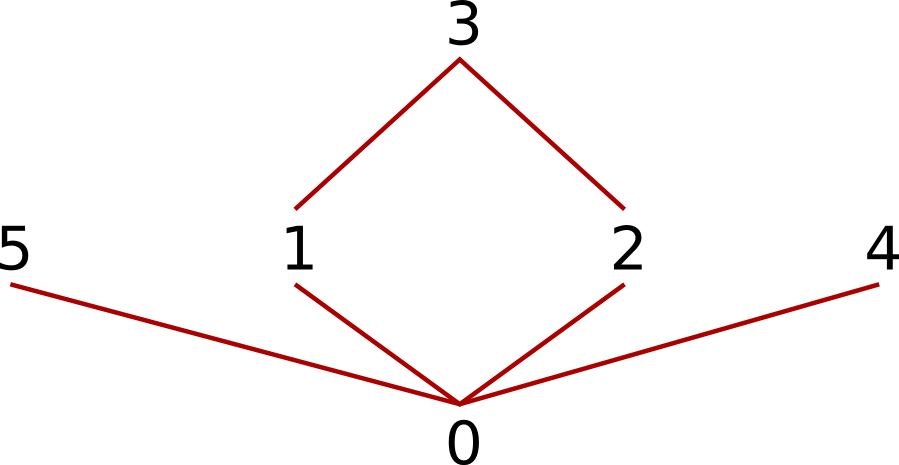
\includegraphics[width=\textwidth]{./figures/sec/secexample_graph.png}%
    }
    \caption{Extracted graph representation of the scene.}
    \label{fig:sec_secexample_graph}
  \end{subfigure}
  \caption{A visualization of an object graph. Computer vision identifies and separates objects and their relative structure to each other (left image). One Semantic Event Graph (right image) results directly from the structure. Please note that multiple roots for one graph are allowed.}
  \label{fig:sec_secexample}
\end{figure}

\begin{align}
  \bordermatrix{
    & 0 & 1 & 2 & 3 & 4 & 5\cr
    0 & \colorbox{green120}{0} & \textup{T} & \textup{T} & \textup{N} & \textup{T} & \textup{T}\cr
    1 & \textup{T} & \colorbox{green120}{1} & \textup{N} & \textup{T} & \textup{N} & \textup{N}\cr
    2 & \textup{T} & \textup{N} & \colorbox{green120}{2} & \textup{T} & \textup{N} & \textup{N}\cr
    3 & \textup{N} & \textup{T} & \textup{T} & \colorbox{green120}{3} & \textup{N} & \textup{N}\cr
    4 & \textup{T} & \textup{N} & \textup{N} & \textup{N} & \colorbox{green120}{4} & \textup{N}\cr
    5 & \textup{T} & \textup{N} & \textup{N} & \textup{N} & \textup{N} & \colorbox{green120}{5}\cr
    },
\end{align}

where ``T'' marks an edge and ``N'' stands for a not-touching relation. 
This matrix is called \gls{ac:sem}.
It is symmetric and contains the object identifiers on the diagonal (marked in green).
Additionally to touching and not-touching, there may be an edge named \emph{absent} ``A'', which is used when new objects come into the scene; for example when a cucumber is being cut into two pieces, or when an object is uncovered during a scene.
Now, each change in the scene corresponds to a change in the touching relation and therefore results in a new matrix. 
A list of \glspl{ac:sem} is called a \acrlong{ac:sec}.
The camera frame, in which the change of relation occurs is called a keyframe.
\Glspl{ac:sec} are independent of the time domain and the robotic hardware. 

\begin{figure}
  \centering
  % Define block styles
\tikzstyle{block} = [rectangle, fill=white, text centered, minimum height=0.5em, rounded corners=true]
\tikzstyle{blockBox} = [draw, rectangle, fill=white, minimum height=3cm, minimum width=4.5cm, text width=1em, text centered, rounded corners=true]

\tikzstyle{blockSupP} = [draw, rectangle, fill=red1!20,   minimum height=0.52cm, minimum width=1.3cm, text width=1em, text centered, rounded corners=true]
\tikzstyle{blockSupM} = [draw, rectangle, fill=green1!20, minimum height=0.52cm, minimum width=4cm, text width=3.8cm, text centered, rounded corners=true]
\tikzstyle{blockSupS} = [draw, rectangle, fill=blue1!20,  minimum height=0.52cm, minimum width=1.3cm, text width=1em, text centered, rounded corners=true]
\tikzstyle{blockSup}  = [draw, rectangle, fill=red1!20,   minimum height=0.52cm, minimum width=3.1cm, text width=3.1cm, text centered, rounded corners=true]

\tikzstyle{blockCon} = [draw, rectangle, fill=white, minimum height=0.5cm, minimum width=1cm, text width=0.6cm, text centered, rounded corners=true]
\tikzstyle{blockP} = [draw, rectangle, fill=red1!40, minimum height=0.52cm, minimum width=0.6cm, text width=1em, text centered, rounded corners=true]
\tikzstyle{blockM} = [draw, rectangle, fill=green1!40, minimum height=0.52cm, minimum width=1.6cm, text width=1.6cm, text centered, rounded corners=true]
\tikzstyle{blockS} = [draw, rectangle, fill=blue1!40, minimum height=0.52cm, minimum width=0.6cm, text width=1em, text centered, rounded corners=true]
\tikzstyle{blockL} = [draw, rectangle, fill=black!20, minimum height=0.52cm, minimum width=0.6cm, text width=1em, text centered, rounded corners=true]
\tikzstyle{arrow} = [draw, -latex]
\tikzstyle{line} = [draw]

\definecolor{red1}{RGB}{160,0,0}
\definecolor{green1}{RGB}{0,160,0}
\definecolor{blue1}{RGB}{0,0,160}

\pgfdeclareimage[width=0.6cm]{hand}{./figures/sec/robothand.jpg}

	      
\begin{tikzpicture}[node distance=6em, auto]
	%%%%%%%%%%%%%%%%%%%%%%%%%%%%%%%%%%%%%%%%%%%%%%%%%%%%%%%%%%%%%%%%%%%%%%%%%%%%%%%%%%%%%%%%%%%%%%%%%%%%%%
	% First line
	\node [blockBox] (p11) {};
	\node [blockBox, right of=p11, node distance=5cm] (p12) {};
	\node [blockBox, right of=p12, node distance=5cm] (p13) {};

	% Panel number
	\node[below left] at (p11.north east) {1};
	\node[below left] at (p12.north east) {2};
	\node[below left] at (p13.north east) {3};

	% Panel 11
	\node[above right, xshift=0.25cm, blockSupM] at (p11.south west) (p11_Sup) {\small{main support (id=0)}};
	\node[above of=p11_Sup, blockM, node distance=0.67cm, xshift=-0.6cm] (p11_m) {\small{m (id=1)}};
	\node[left of=p11_m, node distance=0.7cm, yshift=1.0cm] (p11_h) {\pgfuseimage{hand}};

	% Panel 12
	\node[above right, xshift=0.25cm, blockSupM] at (p12.south west) (p12_Sup) {\small{main support (id=0)}};
	\node[above of=p12_Sup, blockM, node distance=0.67cm, xshift=-0.6cm] (p12_m) {\small{m (id=1)}};
	\node[left of=p12_m, node distance=1.2cm, yshift=0.3cm] (p12_h) {\pgfuseimage{hand}};

	\node[above of=p12_Sup, blockM, node distance=0.67cm, xshift=-0.6cm] (p12_m) {\small{m (id=1)}};

	% Panel 13
	\node[above right, xshift=0.25cm, blockSupM] at (p13.south west) (p13_Sup) {\small{main support (id=0)}};
	\node[above of=p13_Sup, blockM, node distance=0.67cm, xshift=0.9cm] (p13_m) {\small{m (id=1)}};
	\node[left of=p13_m, node distance=1.5cm, yshift=0.9cm] (p13_h) {\pgfuseimage{hand}};

  % Trajectory
  %\draw[dashed, line width=0.25mm] ([xshift=-1.4cm, yshift=1.3cm]p11_Sup.north) to[rounded corners=20pt] ([xshift=-2.1cm, yshift=0.5cm]p11_Sup.north) to[rounded corners=20pt] ([xshift=0.0cm, yshift=0.5cm]p11_Sup.north) to[rounded corners=20pt] ([xshift=-0.6cm, yshift=1.2cm]p11_Sup.north);

  \draw[dashed, line width=0.25mm] ([xshift=-1.4cm, yshift=1.3cm]p12_Sup.north) to[rounded corners=20pt] ([xshift=-1.8cm, yshift=0.7cm]p12_Sup.north);

  \draw[dashed, line width=0.25mm] ([xshift=-1.4cm, yshift=1.3cm]p13_Sup.north) to[rounded corners=20pt] ([xshift=-2.1cm, yshift=0.5cm]p13_Sup.north) to[rounded corners=20pt] ([xshift=0.0cm, yshift=0.5cm]p13_Sup.north) to[rounded corners=20pt] ([xshift=-0.6cm, yshift=1.2cm]p13_Sup.north);


	%%%%%%%%%%%%%%%%%%%%%%%%%%%%%%%%%%%%%%%%%%%%%%%%%%%%%%%%%%%%%%%%%%%%%%%%%%%%%%%%%%%%%%%%%%%%%%%%%%%%%%
	% Second line

  \node[block, below of=p11,    node distance=4.5cm] (p21_ms) {main support, id=0};
  \node[block, above of=p21_ms, node distance=1cm] (p21_m) {main, id=1};
  \node[block, above of=p21_ms, node distance=2cm] (p21_hand) {robot hand, id=2};
  \draw[line] (p21_ms.north) to (p21_m.south);

  \node[block, below of=p12,    node distance=4.5cm] (p22_ms) {main support, id=0};
  \node[block, above of=p22_ms, node distance=1cm] (p22_m) {main, id=1};
  \node[block, above of=p22_ms, node distance=2cm] (p22_hand) {robot hand, id=2};
  \draw[line] (p22_ms.north) to (p22_m.south);
  \draw[line] (p22_m.north) to (p22_hand.south);

  \node[block, below of=p13,    node distance=4.5cm] (p23_ms) {main support, id=0};
  \node[block, above of=p23_ms, node distance=1cm] (p23_m) {main, id=1};
  \node[block, above of=p23_ms, node distance=2cm] (p23_hand) {robot hand, id=2};
  \draw[line] (p23_ms.north) to (p23_m.south);


	%%%%%%%%%%%%%%%%%%%%%%%%%%%%%%%%%%%%%%%%%%%%%%%%%%%%%%%%%%%%%%%%%%%%%%%%%%%%%%%%%%%%%%%%%%%%%%%%%%%%%%
	% Third line

    \node[block, below of=p21_ms, node distance=2.25cm] (p31) {
      $\bordermatrix{
        & 0 & 1 & 2\cr
        0 & \colorbox{green120}{0}  & \textup{T}              & \textup{N}\cr
        1 & \textup{T}              & \colorbox{green120}{1}  & \textup{N}\cr
        2 & \textup{N}              & \textup{N}              & \colorbox{green120}{2}\cr        
      }$
    };

    \node[block, below of=p22_ms, node distance=2.25cm] (p31) {
      $\bordermatrix{
        & 0 & 1 & 2\cr
        0 & \colorbox{green120}{0}  & \textup{T}              & \textup{N}\cr
        1 & \textup{T}              & \colorbox{green120}{1}  & \textup{T}\cr
        2 & \textup{N}              & \textup{T}              & \colorbox{green120}{2}\cr        
      }$
    };

    \node[block, below of=p23_ms, node distance=2.25cm] (p31) {
      $\bordermatrix{
        & 0 & 1 & 2\cr
        0 & \colorbox{green120}{0}  & \textup{T}              & \textup{N}\cr
        1 & \textup{T}              & \colorbox{green120}{1}  & \textup{N}\cr
        2 & \textup{N}              & \textup{N}              & \colorbox{green120}{2}\cr        
      }$
    };
\end{tikzpicture}

  \caption{An example showing a pushing action in the \gls{ac:sec} domain. The first row shows a pictogram view of the action. The \emph{main} object, denoted with ``m'', sits on top the ``main support'' and the robot is not touching the \emph{main} object. In the second keyframe the robot touches the \emph{main} object and pushes it to the right. The robot's trajectory is marked with a dashed line. However, this trajectory information is not encoded in the \gls{ac:sec}. In the third keyframe the robot hand is removed from the \emph{main} object. The middle row holds a graph representation of the touching and not-touching relations; touching relations are marked with a line. In the bottom row the graph is represented as \glspl{ac:sem}. All three matrices hold a lot of static information. Therefore, a short form, which removes all static information, is introduced. For this example one could also write: ``main object -- robot hand: N~T~N''.}
  \label{fig:sec_examplescenario_pushing}
\end{figure}

A second (and also artificial) example of a \action{pushing} action is shown in \figref{fig:sec_examplescenario_pushing}.
A robot pushes the \emph{main} object ``m'' along its support.
In the first keyframe, there is only one touching connection between the object and its support, which is shown in the graph below the pictogram and also reflected in the \gls{ac:sem} below the graph.
Next, the robot begins to touch the \emph{main} object and holds that connection for the entire trajectory, \ie for a longer period of time.
The last (third) keyframe is generated as soon as the robot looses contact to the \emph{main} object.

A third example of a \action{pick and place} action is displayed in \figref{fig:sec_examplescenario_pickandplace}; it is derived from a real world experiment.
In the first keyframe an apple is on top of a plate and the robot hand hovers above the table.
In the next keyframes it holds the apple, lifts it off the plate, and places it on the table.
This sequence of touching/non-touching relations is unique for this type of action.
If in this scene the robot were to push the apple on the plate, the graph sequence would look differently.
While the first two keyframes would look like the pick-and-place example, the third keyframe would be equal to the first: The robot hand hovering in the air.
Immediately one problem becomes apparent: In both examples the first two keyframes are alike, even though in one example the apple is picked and in another example it is pushed.
Therefore, reliable action recognition is only possible on a very late stage of action execution.

\begin{figure}[]
  \centering
  \begin{subfigure}[t]{0.475\textwidth}
    \centering
    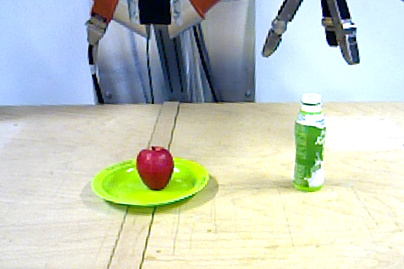
\includegraphics[width=\textwidth]{./figures/sec/scenario/darktable_exported/frame0493.jpg}
    \subcaption{Keyframe 1, this is the very first camera frame.}
    \label{fig:sec_examplescenario_pickandplace_1j}
  \end{subfigure}
  \hfil
  \begin{subfigure}[t]{0.475\textwidth}
    \centering
    % Define block styles
\tikzstyle{block} = [rectangle, fill=white, text centered, rounded corners]
\tikzstyle{arrow} = [draw]
\usetikzlibrary{matrix}

\pgfdeclareimage[width=11em]{ImBlock}{./figures/sec/secexample_blocksmarkednumbered.jpg}
\pgfdeclareimage[width=11em]{ImGraph}{./figures/sec/secexample_graph.png}

\definecolor{red1}{RGB}{160,0,0}
\definecolor{green1}{RGB}{0,160,0}
\definecolor{blue1}{RGB}{0,0,160}

	      
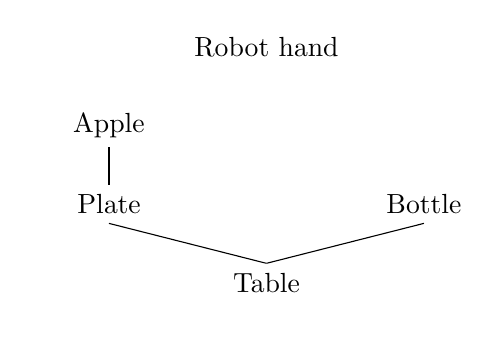
\begin{tikzpicture}[node distance=1cm, auto]
    \node[block] (table) {Table};
    \node[block, above of=table, xshift=-2cm, color=white] (appleW) {Robot hand};

    \node[block, above of=table, xshift=2cm] (bottle) {Bottle};
    \node[block, above of=table, xshift=-2cm] (plate) {Plate};
    \node[block, above of=plate] (apple) {Apple};
    \node[block, above of=apple, xshift=2cm] (hand) {Robot hand};

    % lines
    \draw [arrow] (table.north) to (plate.south);
    \draw [arrow] (table.north) to (bottle.south);
    \draw [arrow] (plate.north) to (apple.south);

    % alignment
    \node[block, below of=table, color=white, node distance=0.4cm] (appleW) {Robot hand};
    \node[block] (table) {Table};
\end{tikzpicture}
%
    \subcaption{Graph representation of Keyframe 1.}
    \label{fig:sec_examplescenario_pickandplace_1t}
  \end{subfigure}\\%
  \begin{subfigure}[t]{0.475\textwidth}
    \centering
    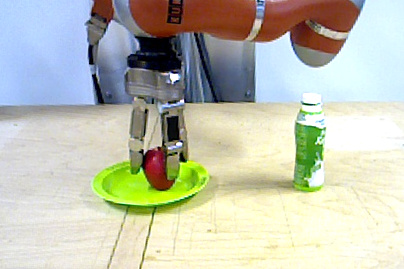
\includegraphics[width=\textwidth]{./figures/sec/scenario/darktable_exported/frame0837.jpg}
    \subcaption{Keyframe 2, the robot arm touches the apple.}
    \label{fig:sec_examplescenario_pickandplace_2j}
  \end{subfigure}
  \hfil
  \begin{subfigure}[t]{0.475\textwidth}
    \centering
    % Define block styles
\tikzstyle{block} = [rectangle, fill=white, text centered, rounded corners]
\tikzstyle{arrow} = [draw]
\usetikzlibrary{matrix}

\pgfdeclareimage[width=11em]{ImBlock}{./figures/sec/secexample_blocksmarkednumbered.jpg}
\pgfdeclareimage[width=11em]{ImGraph}{./figures/sec/secexample_graph.png}

\definecolor{red1}{RGB}{160,0,0}
\definecolor{green1}{RGB}{0,160,0}
\definecolor{blue1}{RGB}{0,0,160}

	      
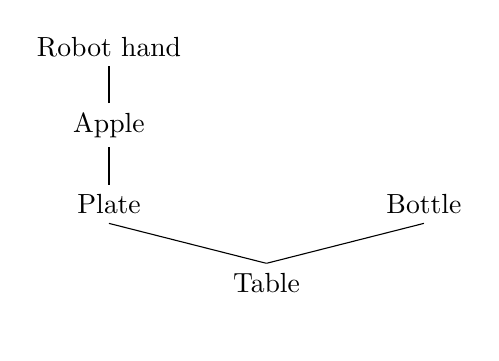
\begin{tikzpicture}[node distance=1cm, auto]
    \node[block] (table) {Table};
    \node[block, above of=table, xshift=-2cm, color=white] (appleW) {Robot hand};

    \node[block, above of=table, xshift=2cm] (bottle) {Bottle};
    \node[block, above of=table, xshift=-2cm] (plate) {Plate};
    \node[block, above of=plate] (apple) {Apple};
    \node[block, above of=apple] (hand) {Robot hand};

    % lines
    \draw [arrow] (table.north) to (plate.south);
    \draw [arrow] (table.north) to (bottle.south);
    \draw [arrow] (plate.north) to (apple.south);
    \draw [arrow] (apple.north) to (hand.south);

    % alignment
    \node[block, below of=table, color=white, node distance=0.4cm] (appleW) {Robot hand};
    \node[block] (table) {Table};
\end{tikzpicture}
%
    \subcaption{Graph representation of Keyframe 2.}
    \label{fig:sec_examplescenario_pickandplace_2t}
  \end{subfigure}\\%
  \begin{subfigure}[t]{0.475\textwidth}
    \centering
    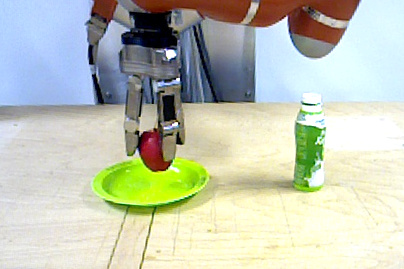
\includegraphics[width=\textwidth]{./figures/sec/scenario/darktable_exported/frame0893.jpg}
    \subcaption{Keyframe 3, the robot lifts the apple of the plate.}
    \label{fig:sec_examplescenario_pickandplace_3j}
  \end{subfigure}
  \hfil
  \begin{subfigure}[t]{0.475\textwidth}
    \centering
    % Define block styles
\tikzstyle{block} = [rectangle, fill=white, text centered, rounded corners]
\tikzstyle{arrow} = [draw]
\usetikzlibrary{matrix}

\pgfdeclareimage[width=11em]{ImBlock}{./figures/sec/secexample_blocksmarkednumbered.jpg}
\pgfdeclareimage[width=11em]{ImGraph}{./figures/sec/secexample_graph.png}

\definecolor{red1}{RGB}{160,0,0}
\definecolor{green1}{RGB}{0,160,0}
\definecolor{blue1}{RGB}{0,0,160}

	      
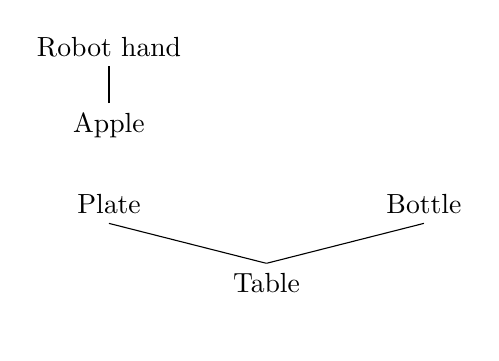
\begin{tikzpicture}[node distance=1cm, auto]
    \node[block] (table) {Table};
    \node[block, above of=table, xshift=-2cm, color=white] (appleW) {Robot hand};

    \node[block, above of=table, xshift=2cm] (bottle) {Bottle};
    \node[block, above of=table, xshift=-2cm] (plate) {Plate};
    \node[block, above of=plate] (apple) {Apple};
    \node[block, above of=apple] (hand) {Robot hand};

    % lines
    \draw [arrow] (table.north) to (plate.south);
    \draw [arrow] (table.north) to (bottle.south);
    \draw [arrow] (apple.north) to (hand.south);

    % alignment
    \node[block, below of=table, color=white, node distance=0.4cm] (appleW) {Robot hand};
    \node[block] (table) {Table};
\end{tikzpicture}
%
    \subcaption{Graph representation of Keyframe 3.}
    \label{fig:sec_examplescenario_pickandplace_3t}
  \end{subfigure}
\end{figure}
\begin{figure}[]\ContinuedFloat
  \centering
  \begin{subfigure}[t]{0.475\textwidth}
    \centering
    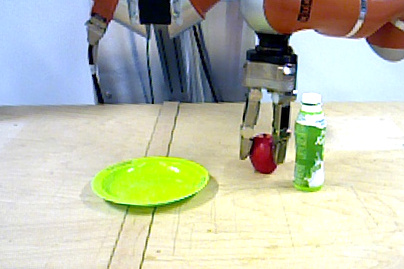
\includegraphics[width=\textwidth]{./figures/sec/scenario/darktable_exported/frame1095.jpg}
    \subcaption{Keyframe 4, the apple is placed on the table.}
    \label{fig:sec_examplescenario_pickandplace_4j}
  \end{subfigure}
  \hfil
  \begin{subfigure}[t]{0.475\textwidth}
    \centering
    % Define block styles
\tikzstyle{block} = [rectangle, fill=white, text centered, rounded corners]
\tikzstyle{arrow} = [draw]
\usetikzlibrary{matrix}

\pgfdeclareimage[width=11em]{ImBlock}{./figures/sec/secexample_blocksmarkednumbered.jpg}
\pgfdeclareimage[width=11em]{ImGraph}{./figures/sec/secexample_graph.png}

\definecolor{red1}{RGB}{160,0,0}
\definecolor{green1}{RGB}{0,160,0}
\definecolor{blue1}{RGB}{0,0,160}

	      
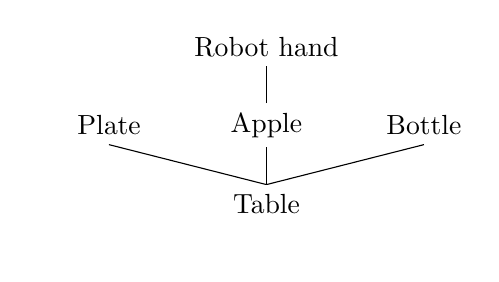
\begin{tikzpicture}[node distance=1cm, auto]
    \node[block] (table) {Table};
    \node[block, above of=table, xshift=-2cm, color=white] (appleW) {Robot hand};

    \node[block, above of=table, xshift=2cm] (bottle) {Bottle};
    \node[block, above of=table, xshift=-2cm] (plate) {Plate};
    \node[block, above of=table] (apple) {Apple};
    \node[block, above of=apple] (hand) {Robot hand};

    % lines
    \draw [arrow] (table.north) to (plate.south);
    \draw [arrow] (table.north) to (bottle.south);
    \draw [arrow] (table.north) to (apple.south);
    \draw [arrow] (apple.north) to (hand.south);

    % alignment
    \node[block, below of=table, color=white, node distance=0.4cm] (appleW) {Robot hand};
    \node[block] (table) {Table};
\end{tikzpicture}
%
    \subcaption{Graph representation of Keyframe 4.}
    \label{fig:sec_examplescenario_pickandplace_4t}
  \end{subfigure}\\%
  \begin{subfigure}[t]{0.475\textwidth}
    \centering
    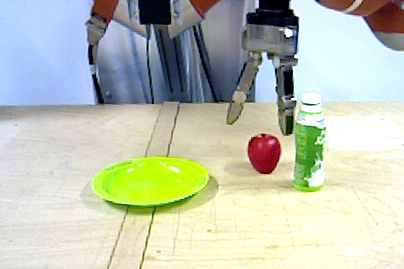
\includegraphics[width=\textwidth]{./figures/sec/scenario/darktable_exported/frame1174.jpg}
    \subcaption{Keyframe 5, the robot arm lets go of the object.}
    \label{fig:sec_examplescenario_pickandplace_5j}
  \end{subfigure}
  \hfil
  \begin{subfigure}[t]{0.475\textwidth}
    \centering
    % Define block styles
\tikzstyle{block} = [rectangle, fill=white, text centered, rounded corners]
\tikzstyle{arrow} = [draw]
\usetikzlibrary{matrix}

\pgfdeclareimage[width=11em]{ImBlock}{./figures/sec/secexample_blocksmarkednumbered.jpg}
\pgfdeclareimage[width=11em]{ImGraph}{./figures/sec/secexample_graph.png}

\definecolor{red1}{RGB}{160,0,0}
\definecolor{green1}{RGB}{0,160,0}
\definecolor{blue1}{RGB}{0,0,160}

	      
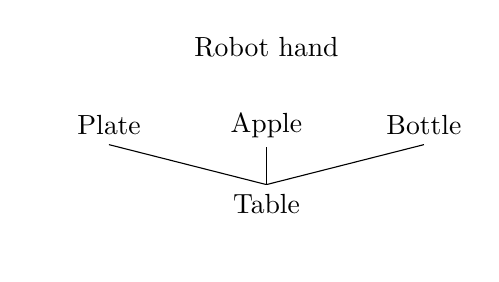
\begin{tikzpicture}[node distance=1cm, auto]
    \node[block] (table) {Table};
    \node[block, above of=table, xshift=-2cm, color=white] (appleW) {Robot hand};

    \node[block, above of=table, xshift=2cm] (bottle) {Bottle};
    \node[block, above of=table, xshift=-2cm] (plate) {Plate};
    \node[block, above of=table] (apple) {Apple};
    \node[block, above of=apple] (hand) {Robot hand};

    % lines
    \draw [arrow] (table.north) to (plate.south);
    \draw [arrow] (table.north) to (bottle.south);
    \draw [arrow] (table.north) to (apple.south);

    % alignment
    \node[block, below of=table, color=white, node distance=0.4cm] (appleW) {Robot hand};
    \node[block] (table) {Table};
\end{tikzpicture}
%
    \subcaption{Graph representation of Keyframe 5.}
    \label{fig:sec_examplescenario_pickandplace_5t}
  \end{subfigure}%
  \caption{Frames from a robot demonstration: The robot picks an apple from a plate and places it on the table. The corresponding graph representation is given on the right side.}
  \label{fig:sec_examplescenario_pickandplace}
\end{figure}

Another problem surfaces, when thinking about the \action{scratching} action: \ie scratching with a robot finger on paper.
This action is indistinguishable from the pushing action on the \gls{ac:sec} domain, they only differ in the robot hands trajectory.
Both actions last for three keyframes where the first and last keyframes are identical; in the second keyframe the robot touches the object.
Here, it is important to note that \glspl{ac:sec} do not store trajectory or time information.
While on the one side this seems like a disadvantage, it is in fact the biggest strength of the \gls{ac:sec} domain.
Trajectory information is hardware dependent and therefore robot specific.
Using \glspl{ac:sec} one can recognize~\cite{aksoytamosiunaitevuga2013}, learn~\cite{aksoy2011learning, aksoydellentamosiunaite2011}, and repeat~\cite{aksoydellentamosiunaite2011} a very wide range of actions.
Furthermore, actions can be enriched using action-related trajectory information and thus be used for bootstrap learning~\cite{aksoytamosiunaitevuga2013}.

Still, not necessarily all actions a human can perform may be encoded using \glspl{ac:sec}.
For some actions higher level knowledge is needed.
As an example of these actions, \action{spreading the marmelade} may serve as an example.
It first depends on the trajectory's velocity and second on the size of the bread, which cannot be described based on \glspl{ac:sec} alone.
To overcome some of these shortcomings of \glspl{ac:sec}, in the next chapter pose information is added.
This will allow for a framework to execute actions, which generalizes while still being independent of the time domain.
